\documentclass[11pt]{article}

\usepackage[margin=1in]{geometry}
\usepackage{amsmath,amssymb}
\usepackage{graphicx}
\usepackage{booktabs}
\usepackage{hyperref}
\usepackage{authblk}
\usepackage{abstract}
\usepackage{natbib}

\hypersetup{
  colorlinks=true,
  linkcolor=blue,
  citecolor=blue,
  urlcolor=blue,
}

\title{The Granularity Ceiling: \\
       Why Pitch-Level Simulation Cannot Beat PA-Level Priors \\
       for Pre-Game MLB Strikeout-Prop Prediction}

\author[1]{Nicholas Matteo}
\affil[1]{Bentley University, Fintech}

\date{\today}

\begin{document}

\maketitle

\begin{abstract}
\noindent We report a negative empirical result on architectures for pre-game
Major League Baseball starting-pitcher strikeout-prop prediction. A pitch-by-pitch
Monte Carlo simulator with five cascaded outcome models (swing, whiff, called
strike, foul, pitch-type arsenal) and a per-count-state calibration layer
scores worse multi-season log loss (0.570) than both a plate-appearance-level
logistic regression with engineered features (0.530) and a naive constant-rate
baseline (0.542). The mechanism is structural rather than implementation-level:
on 241 holdout pitchers with $\geq 50$ test plate appearances, the simulator's
per-pitcher implied K rate correlates $r = 0.38$ with realized K rate versus
$r = 0.58$ for a Beta-shrunk as-of cumulative prior; the simulator's estimate
standard deviation is compressed 42\% versus the realized std (0.031 vs 0.053),
the empirical signature of mean shrinkage. The result is consistent with a Central Limit Theorem
washout argument: at start-level aggregation across $\sim$24 plate appearances,
within-AB pitch sequencing structure averages out, and what survives is the
per-AB mean K probability. The pitch-level outcome models, trained on
league-wide radar-gun physics and arsenal mix, cannot recover the
unobservable per-pitcher skill component (deception, tunneling, pitch shape
similarity) that the cumulative prior captures directly from observed outcomes.
We argue that this implies a general principle for aggregated prediction
problems: microstructure modeling cannot improve aggregate prediction quality
beyond what the microstructure model achieves on per-unit mean estimation.
The result generalizes to pre-game options pricing, NFL play-level statistics,
season-level win totals, and other domains where the bet unit aggregates over
many micro-units.
\end{abstract}

\section{Introduction}

\section{Background}

\subsection{MLB Strikeout Props}
\subsection{Plate-Appearance Level Baseline}
\subsection{Sharp-Book Reference}

\section{The Pitch-Level Architecture}

\subsection{Component Models}
\subsection{Vectorized AB Simulator}
\subsection{Per-Count-State Calibration}

\section{Results}

\subsection{Headline Comparison}

\begin{table}[h]
\centering
\caption{Multi-season K log loss by architecture (lower is better).}
\begin{tabular}{lrr}
\toprule
Architecture & Log Loss & MAE \\
\midrule
Constant-rate baseline       & 0.5422 & 1.83 \\
PA logistic + features (M1--M7) & \textbf{0.5300} & 1.78 \\
PA simulator                  & 0.5367 & 1.79 \\
PA simulator + calibration    & 0.5342 & 1.78 \\
Pitch-level simulator         & 0.5702 & 1.93 \\
\bottomrule
\end{tabular}
\end{table}

\subsection{Per-Pitcher Correlation Diagnostic}

\begin{table}[h]
\centering
\caption{Per-pitcher implied K-rate estimator vs realized K rate on the
chronological holdout. $n = 241$ pitchers with $\geq 50$ test plate appearances.}
\begin{tabular}{lrrr}
\toprule
Estimator & Pearson $r$ & MAE & Std of estimate \\
\midrule
Beta-shrunk as-of prior        & 0.576 & 0.036 & 0.038 \\
Pitch-sim per-pitcher average  & 0.378 & 0.041 & 0.031 \\
Realized (ground truth)        & 1.000 & 0.000 & 0.053 \\
\bottomrule
\end{tabular}
\end{table}

\begin{figure}[h]
\centering
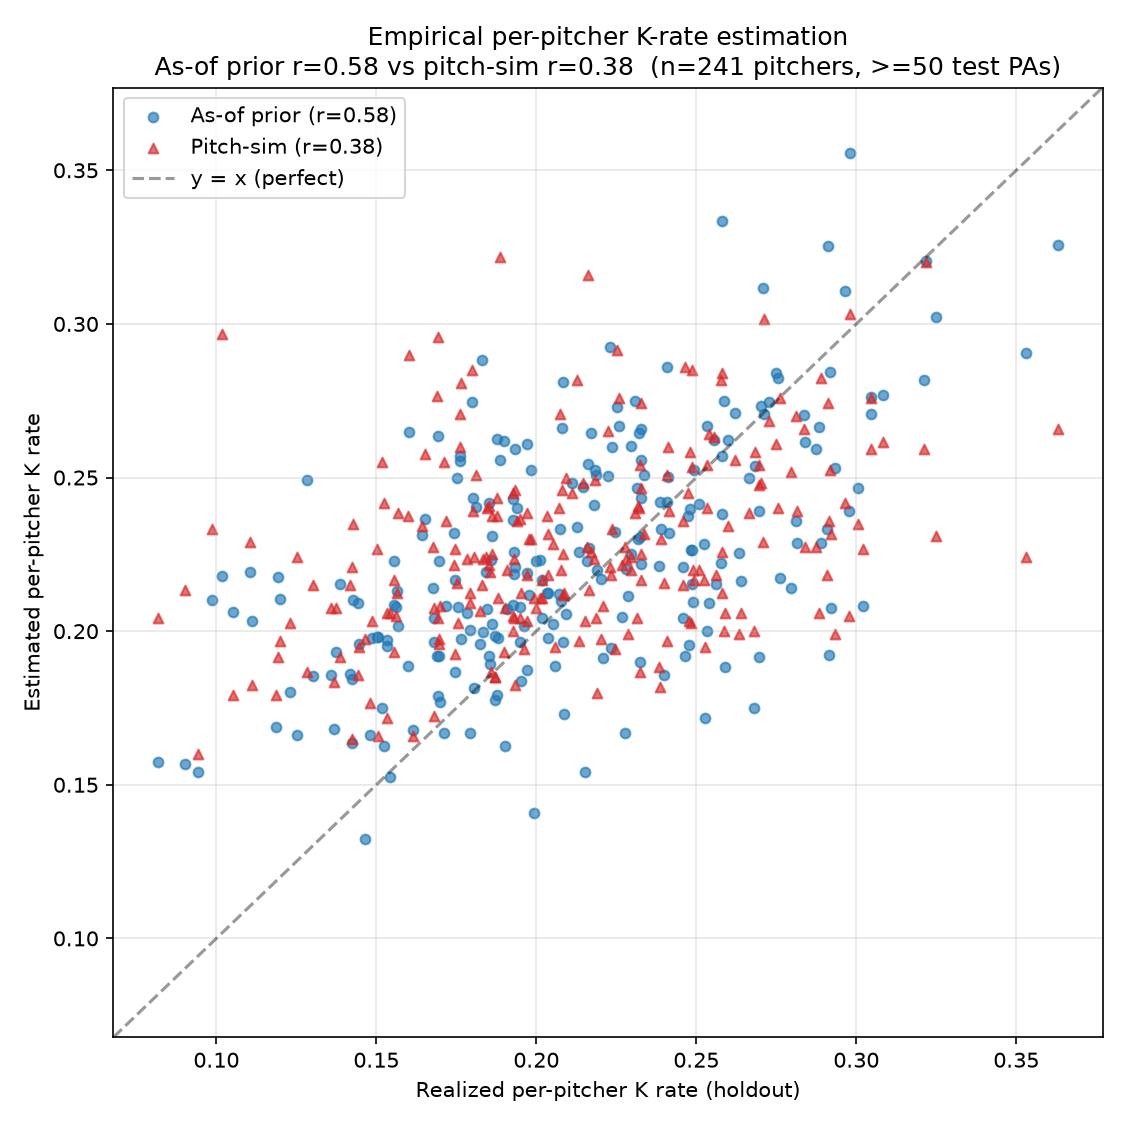
\includegraphics[width=0.75\linewidth]{../figures/correlation_scatter_empirical.png}
\caption{Per-pitcher K rate estimation on the empirical holdout ($n = 241$
pitchers, $\geq 50$ test plate appearances). The as-of prior (blue) recovers
the realized skill spread; the pitch-level simulator (red) shrinks predictions
toward the league mean (the empirical signature of mean shrinkage).}
\end{figure}

\begin{figure}[h]
\centering
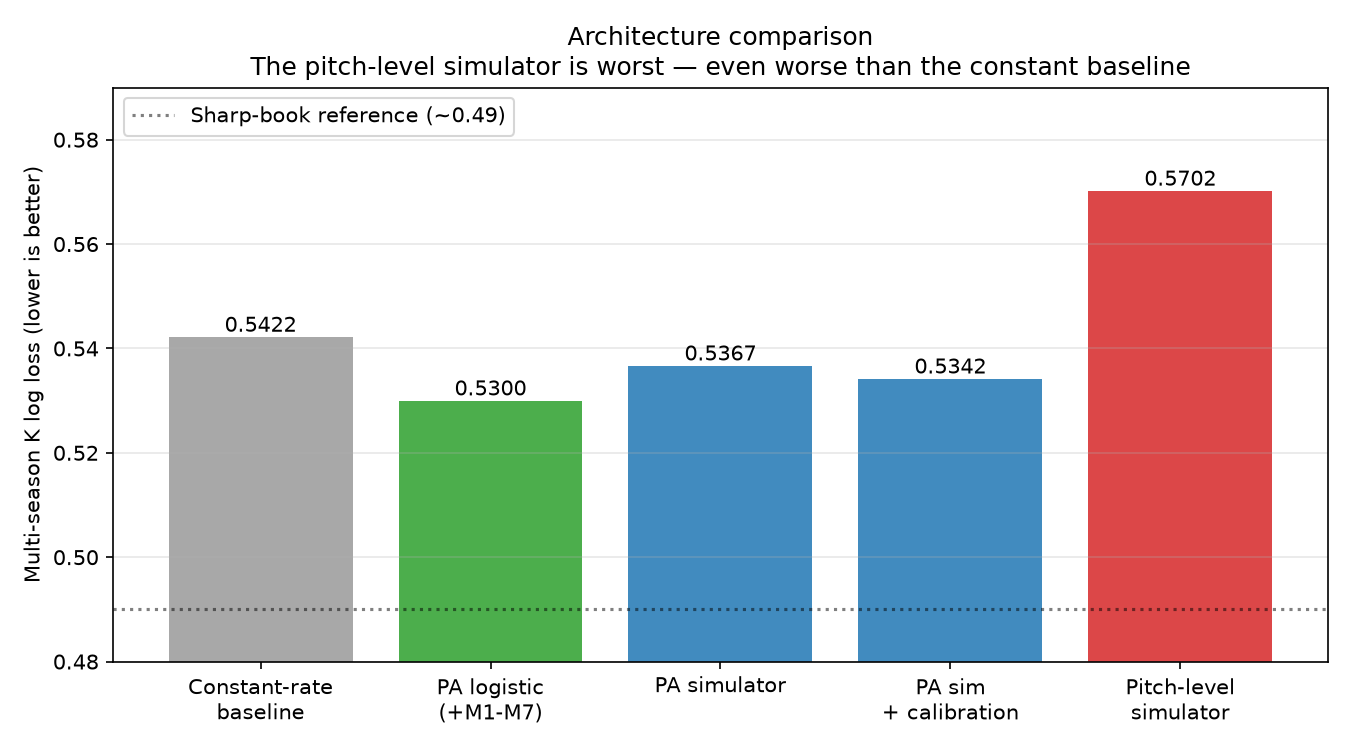
\includegraphics[width=0.85\linewidth]{../figures/log_loss_bar.png}
\caption{Architecture comparison on multi-season K log loss. The pitch-level
simulator is worst, including vs the constant-rate baseline.}
\end{figure}

\section{Mechanism: Central Limit Theorem Washout}

\section{Generalization to Other Aggregated Prediction Domains}

\section{Reproducibility}

\section{Conclusion}

\bibliographystyle{plainnat}
\bibliography{references}

\end{document}
